
%\documentclass[options]{class}
\documentclass[10pt,journal]{IEEEtran}

%Paquete de Idioma
\usepackage[spanish]{babel}
\usepackage{graphicx}

%Codificación Alfabeto
\usepackage[utf8]{inputenc}
\usepackage{amsmath}
\usepackage{amsfonts}
\usepackage{amssymb}
%\usepackage{amstext} 

%Codificación de Fuente
\usepackage[T1]{fontenc}

%Estilo de Página Numeración superior
%\pagestyle{headings}

%Hiperlinks \href{url}{text}
\usepackage[pdftex]{hyperref}

\usepackage{graphicx}

\begin{document}

%Titulo
\title{Determinación de la longitud focal de lentes delgadas}

%Autor
\author{Fernando Dalai Aguilar Sánchez \\ Laboratorio de óptica, ESFM-IPN, Ciudad de México, México \\21 marzo de 2023}


\maketitle{}  

%Resumen
\begin{abstract}
En esta práctica de laboratorio se utilizaron tres métodos diferentes para medir la distancia focal de una lente delgada. El objetivo fue determinar cuál de los métodos es el más preciso y confiable. El método directo se realizó utilizando un láser y una pantalla, mientras que el método de autocolimación consistió en variar la distancia entre la lente y las rendijas hasta obtener una imagen nítida. El método del doble desplazamiento implicó deslizar la lente a una segunda posición para obtener una segunda imagen nítida. Los resultados obtenidos de los tres métodos se compararon
\end{abstract}  

\section{Introducción}
La lente delgada es un componente óptico utilizado para desviar, enfocar o dispersar los rayos de luz que atraviesan su superficie refringente. Estas lentes son dispositivos ópticos simétricos, que se componen de dos superficies refringentes separadas por un material dieléctrico homogéneo, y tienen la propiedad de cambiar la trayectoria de los rayos de luz que pasan a través de ellas.

Las lentes delgadas se clasifican en lentes convergentes o positivas y lentes divergentes o negativas, dependiendo de si su poder óptico hace que los rayos de luz converjan o diverjan después de atravesarlas. Las lentes convergentes tienen una forma de curvatura convexa, mientras que las lentes divergentes tienen una forma de curvatura cóncava.

La capacidad de una lente para enfocar los rayos de luz se mide en términos de su distancia focal, que es la distancia desde la lente hasta el punto focal, donde los rayos paralelos se cruzan después de atravesar la lente. La distancia focal depende de la forma de la lente, su índice de refracción y la distancia de la fuente de luz a la lente.

Las lentes delgadas también tienen una ecuación matemática que describe su comportamiento óptico. Esta ecuación se conoce como la ecuación de la lente delgada y se puede expresar en formato LaTeX de la siguiente manera:

\begin{equation}
\frac{1}{f} = \frac{1}{d_o} - \frac{1}{d_i}
\end{equation}.

donde f es la distancia focal de la lente, $d_o$ es la distancia del objeto a la lente y $d_i$ es la distancia de la imagen a la lente.


\begin{figure}[!ht]
\begin {center}
\includegraphics[width=0.4\textwidth]{5.png}
\caption{Lente positiva}
\end {center}
\end{figure}

\begin{figure}[!ht]
\begin {center}
\includegraphics[width=0.4\textwidth]{6.png}
\caption{Lente negativa}
\end {center}
\end{figure}


\section{Metodología}


\subsection{Método directo}
Con el objetivo de determinar la distancia focal de una lente, procedimos a utilizar un láser y una óptica de expansión del rayo. En primer lugar, hicimos incidir el haz del láser sobre la lente y movimos la pantalla hasta que logramos obtener un punto nítido sobre la misma. De esta manera, pudimos asegurarnos de que habíamos localizado el punto focal de la lente. A continuación, medimos la distancia desde la lente hasta la pantalla, lo que nos permitió determinar la distancia focal.

Para confirmar nuestros resultados, giramos la lente y presentamos la otra cara a la incidencia del rayo láser, y repetimos el procedimiento. De esta forma, pudimos obtener una medida más precisa de la distancia focal de la lente.




\begin{figure}[!ht]
\begin {center}
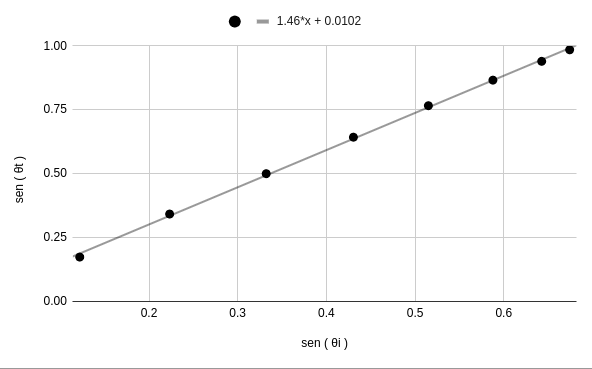
\includegraphics[width=0.4\textwidth]{2.jpeg}
\caption{Método directo}
\end {center}
\end{figure}

\subsection{Método de autocolimación} 

variamos la distancia entre las lentes y las rendijas hasta que obtuvimos una imagen nítida de las rendijas al lado de las rendijas. Con esto garantizamos que la distancia entre las lentes y las rendijas era igual a la distancia focal.

Fue interesante observar cómo al variar la distancia entre la lente y la rendija, la imagen proyectada también variaba, y era necesario hacer pequeños ajustes para lograr la nitidez deseada. Nos tomó varios intentos encontrar la posición óptima de las lentes, pero finalmente logramos obtener una imagen clara y definida.

Después de este primer paso, giramos las lentes para que presentaran la otra cara a la incidencia y repetimos el procedimiento. Esta vez, gracias a nuestra experiencia previa, el proceso fue más rápido y logramos obtener una imagen clara en menos intentos.

\begin{figure}[!ht]
\begin {center}
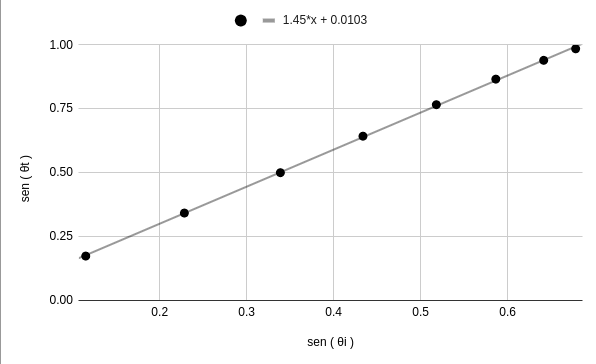
\includegraphics[width=0.4\textwidth]{4.jpeg}
\caption{Método de autocolimación}
\end {center}
\end{figure}


\subsection{Método del Doble Desplazamiento} 

Una vez que habíamos preparado el montaje experimental, nuestro siguiente paso fue encontrar la imagen nítida de la rendija en la pantalla. Con paciencia y precisión ajustamos la lente hasta lograr el enfoque adecuado.

Después, nos propusimos deslizar la lente hasta la segunda posición en donde también pudiéramos encontrar una imagen nítida de la rendija en la pantalla. Fue un proceso meticuloso, pero al final lo logramos.

Una vez que obtuvimos ambas imágenes, medimos la distancia de la lente entre posición uno y dos. Esta distancia, conocida como "d", era fundamental para nuestros cálculos posteriores y para obtener los resultados que estábamos buscando.

\begin{figure}[!ht]
\begin {center}
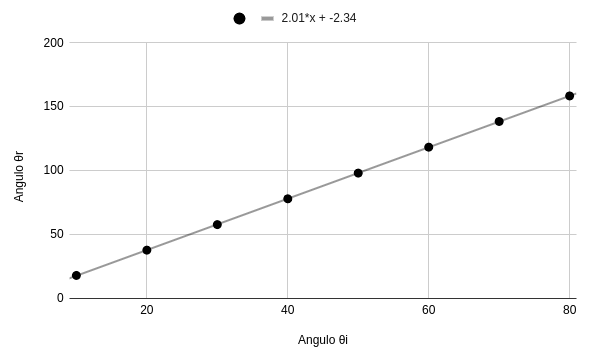
\includegraphics[width=0.4\textwidth]{3.jpeg}
\caption{Método del doble desplazamiento}
\end {center}
\end{figure}

\section{Resultados}


%\subsection{Método directo}


Para el primer método (Directo) se obtuvieron los siguientes datos para las lentes de 100 mm y 50 mm respectivamente:
\begin{center}
\begin{tabular}{|c|c|c|}
\hline
N & fe(mm) & ff(mm) \\
\hline
1 & 105 & 100\\
\hline
2 & 99 & 100\\
\hline
3 & 99 & 100\\
\hline
4 & 101 & 100\\
\hline
5 & 50 & 50\\
\hline
6 & 53 & 50\\
\hline
7 & 60 & 50\\
\hline
8 & 56 & 50\\
\hline
\end{tabular}
\end{center}

En  el caso del método de autocolimación se obtuvó:

\begin{center}
\begin{tabular}{|c|c|c|}
\hline
N & fe(mm) & ff(mm) \\
\hline
1 & 189 & 100\\
\hline
2 & 199 & 100\\
\hline
3 & 196 & 100\\
\hline
4 & 196 & 100\\
\hline
5 & 202 & 50\\
\hline
6 & 200 & 50\\
\hline
7 & 201 & 50\\
\hline
8 & 202 & 50\\
\hline
\end{tabular}
\end{center}


Para el tercer método tenemos:

\begin{center}
\begin{tabular}{|c|c|c|c|}
\hline
N & d(cm) & D(cm) & ff(mm) \\
\hline
1 & 45.5 & 100 & 200 \\
\hline
2 & 39.8 & 90 & 200 \\
\hline
3 & 58 & 110 & 200\\
\hline
4 & 75 & 120 & 200\\
\hline
\end{tabular}
\end{center}


\section{Discusión y conclusiones}

Se ha llevado a cabo una comparación de los resultados obtenidos mediante tres métodos diferentes para la medición de la distancia focal de una lente. Después de analizar los datos, se ha llegado a la conclusión de que el método de autocolimación es el más confiable para obtener mediciones precisas y cercanas al valor de fabricación. Este método ha presentado el menor error porcentual de los tres métodos utilizados, lo que sugiere que es el más preciso y confiable para la medición de la distancia focal.

No obstante, se ha observado que los tres métodos son viables para lograr el objetivo de la práctica, lo que indica que cualquier método podría ser utilizado para este propósito. A pesar de esto, es importante destacar que los errores obtenidos en las mediciones podrían haber sido causados por errores instrumentales o humanos en las mediciones realizadas en cada experimentación.

En conclusión, se sugiere realizar nuevas mediciones más precisas para obtener mediciones más confiables y cercanas al valor de fabricación de la lente. De esta manera, se puede minimizar la influencia de los errores instrumentales y humanos en las mediciones y mejorar la precisión de los resultados obtenidos.

\section{Bibliografía}


Resnick, Halliday y Krane, (2002). Física. VOl I. México. Editorial Cecsa.


Serway, R.A., Jewett, J.W. (2009). "Física: Para ciencia e ingeniería con Física Moderna", 7 Edicion. Vol.2 México. Cengage.


W. Sears, MW Zemansky, HD Young y R. A. Freedman: "Física universitaria", 12 Edición. VOl 2. Addison-Wesley-Longman/Pearson Education.



\end{document}
